In disk-based databases, I/O is the bottleneck, therefore the volume
of data moved from disk to memory (and back) is a good indication of
algorithm efficiency. Disk-based algorithms are designed to work with
large data volumes in a "slow" medium (disk) by temporarily storing
small parts in a vastly faster medium (main memory) and writing them
back when processing is done. In some cases data has to be written
back to a temporary file on disk, further increasing I/O-traffic.

\begin{figure}[H]
	\centering
	% left bottom right top
	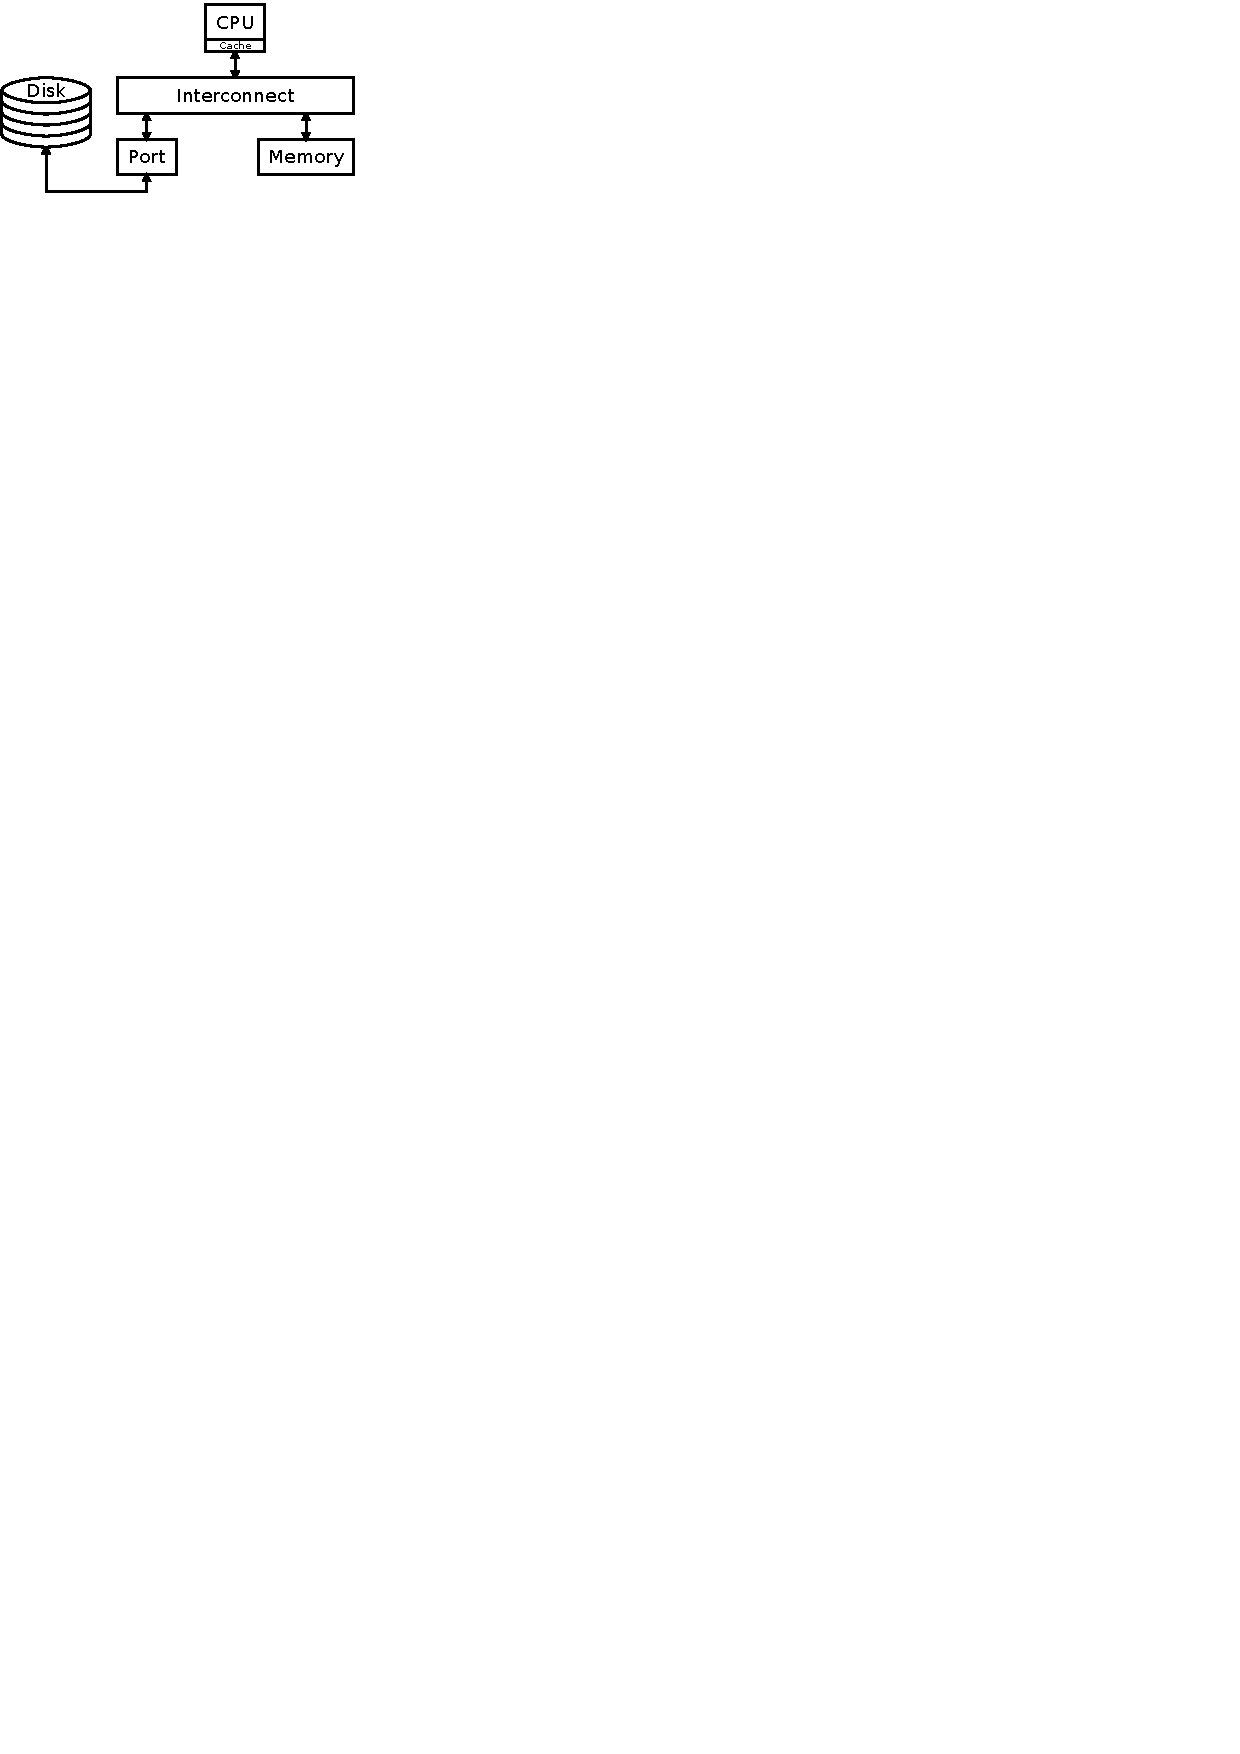
\includegraphics[scale=1.5,trim=0 26.45cm 15.05cm 0.1cm]{img/disk-based-architecture}
	\caption{Disk-based architecture}
	\label{fig:disk-based-arch}
\end{figure}

Figure \ref{fig:disk-based-arch} shows a simplified view of the target
architecture. The processor is connected to disk and memory by an
interconnect bus. Disk has an extra layer before the interconnect,
this can be PCI or similar, generally described as an external bus.
Communicating with main memory is a relatively fast operation, data is
transferred over the internal bus (interconnect), while disk
communication needs to be sent through an external bus, in addition to
waiting for a slower medium (typically a magnetic hard disk drive
requiring mechanical motion to access data).

There are three main groups of disk-based methods: nested loop,
sorting, and partitioning. Additionally, indexes, filters, histograms
and other methods are used to improve performance.

\section{Nested loop}

Nested loop (NL) is the most straight-forward method, it is very
efficient for small to moderate operand volumes \cite{bratbergsengen}.
This method exploits main memory to save CPU and I/O work by
temporarily storing records in a workspace (WS) during execution.
Using a big workspace will give improved performance. Ideally WS is
big enough to hold the entire input relation A. This method is
outlined in Algorithm \ref{alg:nested-loop}, upper case letters are
relations while lower case are records. Note that the smallest input
relation, A, is used in outer loop to minimize I/O-traffic.

\begin{algorithm}
	\caption{Nested loop}
	\label{alg:nested-loop}
	\begin{algorithmic}
		\REQUIRE A = smallest input relation, B = bigger 
		(or equally sized) input relation, R = output relation
		\ENSURE R contains result of algebra operation
		\WHILE{A has unread records}
			\STATE{read records from A and store in WS until WS is full or A is read}
			\FORALL{$b \in B$}
				\IF{$b \in A$}
					\STATE complete algebra operation for record b and
					save result to R
				\ENDIF
			\ENDFOR
		\ENDWHILE
	\end{algorithmic}
\end{algorithm}

The workspace structure is a critical part of this method, and it
should be optimized for fast access to records when complete key is
known. Bratbergsengen use a combination of hashing and binary trees in
\cite{bratbergsengen}. Hashing partitions keys into smaller sets and
binary trees give a reasonable search length, even if hash
partitioning fails. Each node consists of four values: left subtree
pointer, right subtree pointer, pointer to record and signature. The
signature can be used to rule out records that does not match a
search, when a potential match is found record key must be read.
Using 4 words (16B) per node provides an additional advantage,
cache-friendliness for architectures where cache-lines are multiples
of 4 words (i.e. the common architectures). Figure \ref{fig:workspace}
illustrates the idea, hash table is depicted at the top, actual tuples
at the bottom, and binary trees between.

\begin{figure}[H]
	\centering
	% left bottom right top
	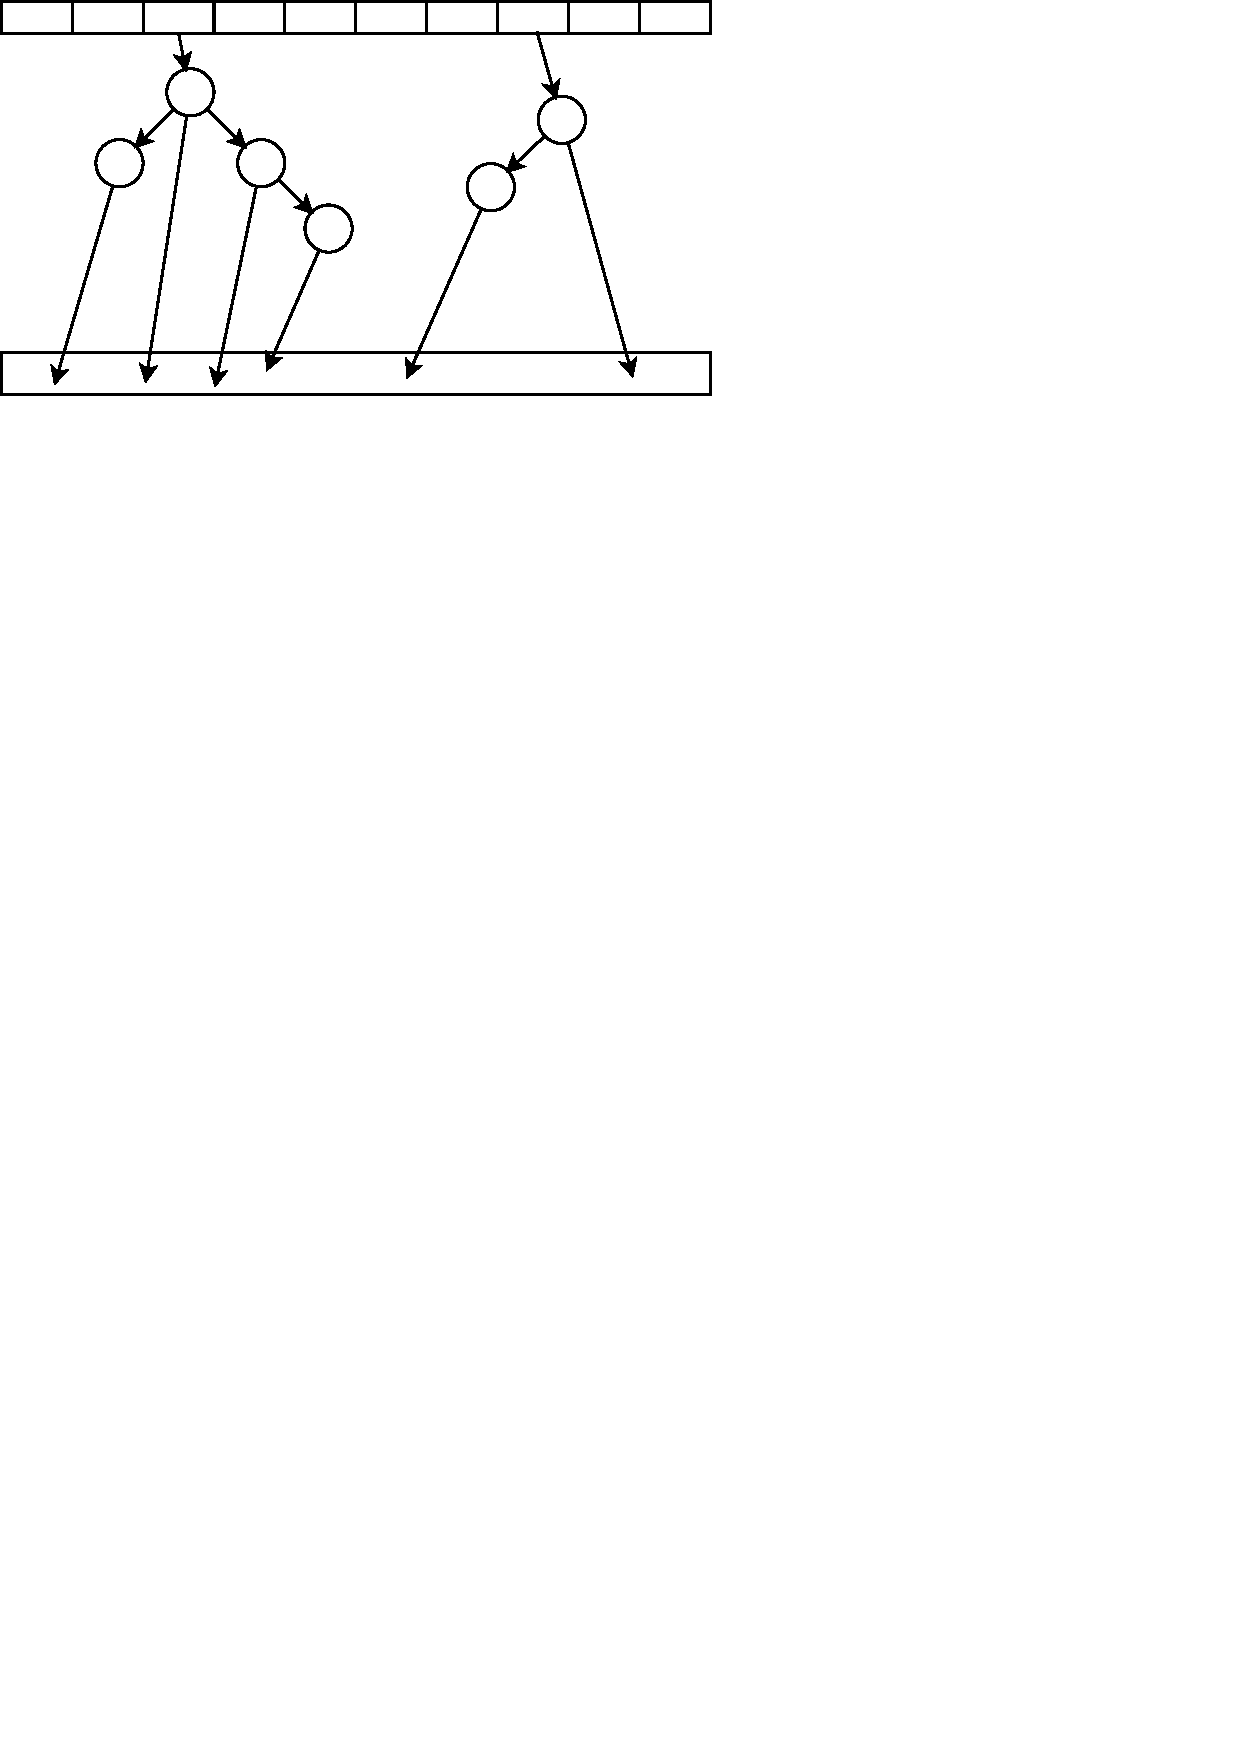
\includegraphics[scale=0.7,trim=0.25 23cm 8.95cm 0.1cm]{img/workspace}
	\caption{Nested loops workspace}
	\label{fig:workspace}
\end{figure}

\section{Sorting}

Sorting method is used to exploit properties of sorted datasets. In
the general case, all input operands are sorted by operation key. If
input are sorted already this can give a performance gain, but for
single operations where no sorting is required, other methods are
likely to be more efficient. For instance, checking for duplicates is
a trivial task if sorted input is available. Latest unique record can
be used to discard all subsequent duplicates without any additional
runs.

\section{Partitioning}
\label{sec:partitioning}

Partitioning is used to prepare input data for nested loop method by
splitting smallest operand into workspace-sized partitions. The goal
is to avoid repeated operand passes, and thereby reduce I/O. An
effective way of partitioning is to use a hash formula that uniformly
distributes data among partitions. Partitions are stored on disk
before nested loop method is executed.

\begin{figure}[H]
	\centering
	% left bottom right top
	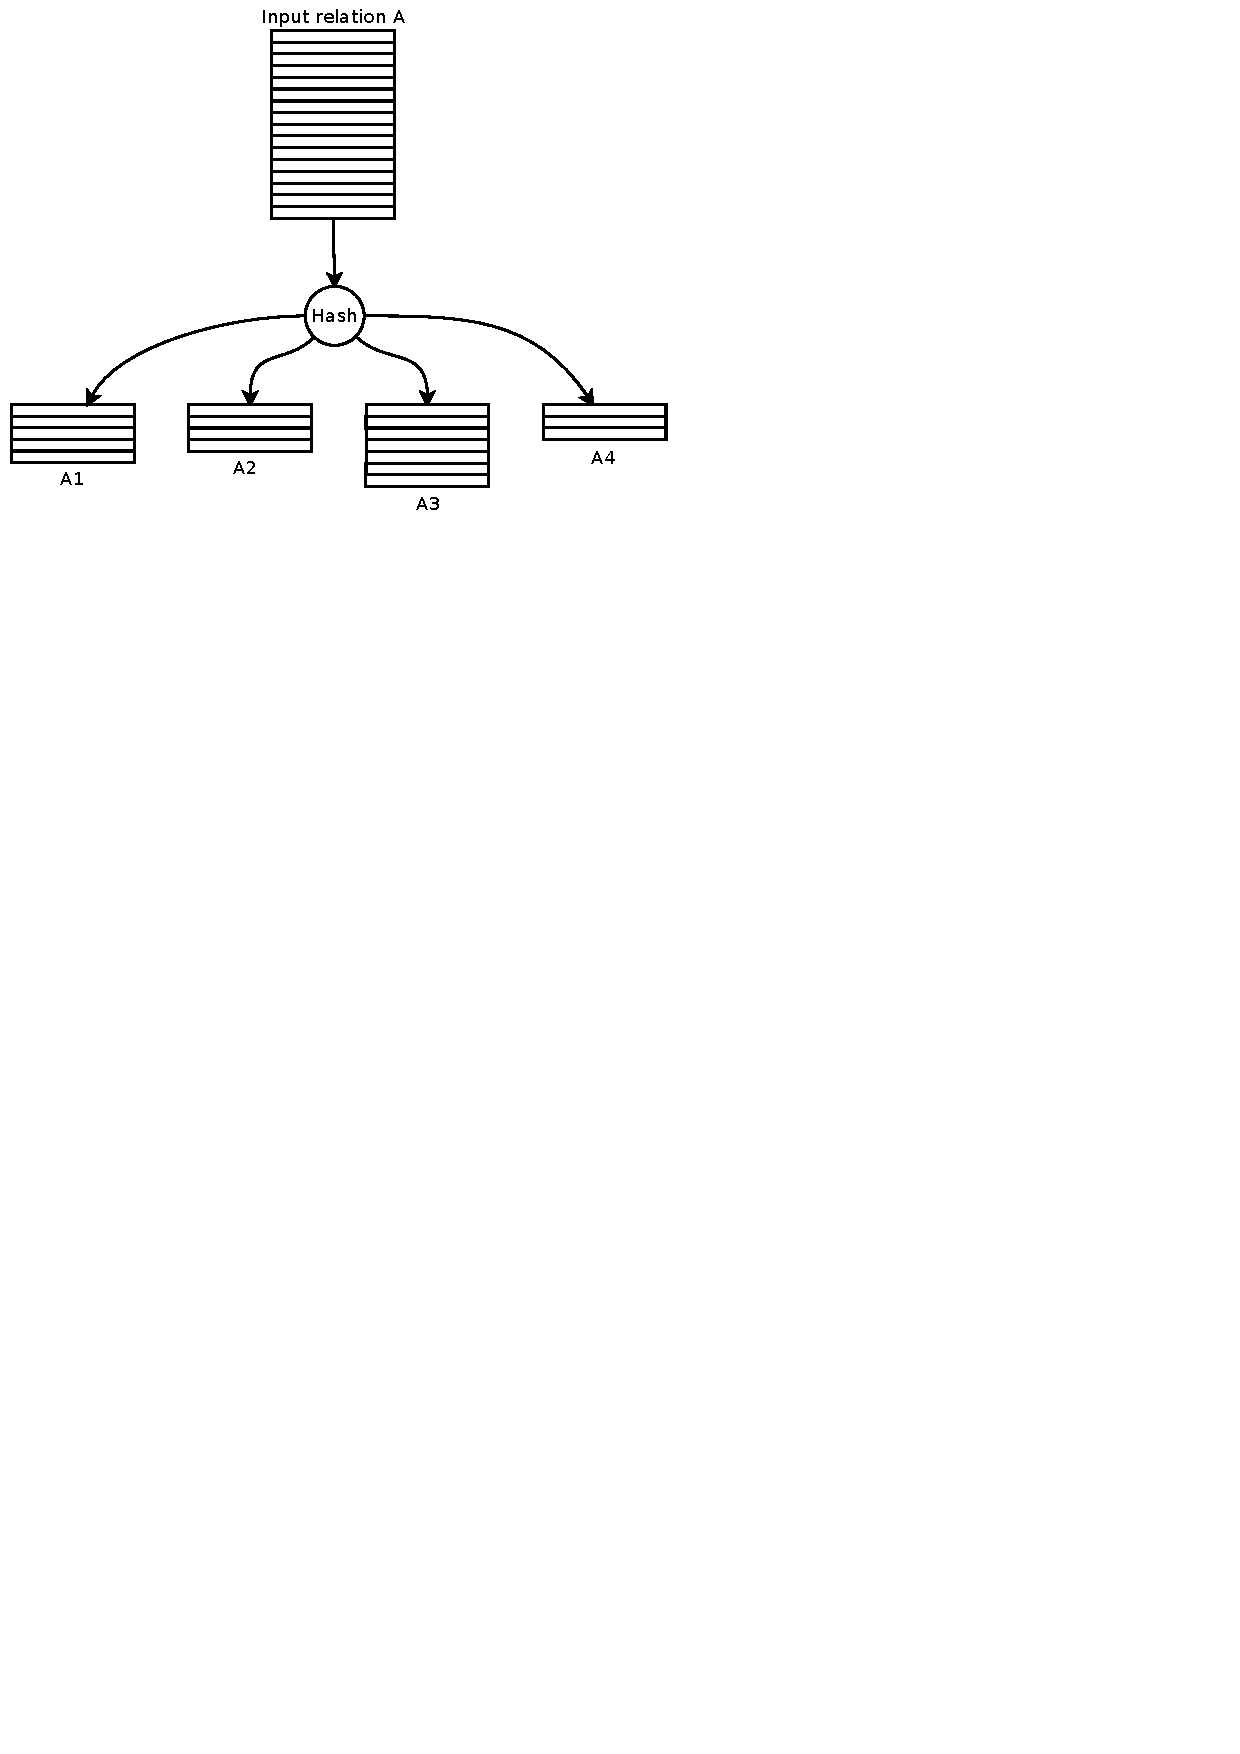
\includegraphics[scale=0.9,trim=0.25cm 21cm 9.80cm 0.1cm]{img/partitioning}
	\caption{Partitioning}
	\label{fig:partitioning}
\end{figure}

Figure \ref{fig:partitioning} illustrates the partitioning of an input
relation A. It is split into four partitions, A1, \ldots, A4 using a
hash function, each partition contains a similar amount of records.
These partitions are in turn fed to the nested loop method, and
results are stored in one relation. The figure also illustrates that
partitions may have different sizes, i.e. a certain degree of skew are
expected. This can be caused by a hash function that are unable to
create a uniform distribution based on the input relation. To ensure
that most groups fit into WS without a perfectly uniform distribution,
nominal group size is normally chosen slightly smaller than WS size
(5-10\%).

\section{Selection and projection}

Selection can be implemented using nested loop by inspecting all
records, and writing matches to the result. If sorted input is
available on the relevant key, only a subset of the input relation
needs to be processed. The problem is reduced to finding the first
match and reading records until there are no more matches.
Partitioning can be utilized for parallel execution by distributing
input relation to different processes (or nodes).

Projection is more involved due to the requirement of returning only
unique records. There are two principal ways to solve this problem
using nested loop:

\begin{enumerate}
	\item Store records in result set on first discovery, and check
	result for duplicate values every time a new records is processed
	\item Fill WS with records from input relation, and subsequently
	remove duplicates from WS by reading the entire relation before
	moving all records in WS to result set, see Algorithm \ref{alg:nl-projection}
\end{enumerate}

\begin{algorithm}
	\caption{NL-Projection}
	\label{alg:nl-projection}
	\begin{algorithmic}
		\REQUIRE A = input relation, 
		P = set of attribute identifiers that should be included in
		result, R = output relation
		\ENSURE R contains no duplicate rows, and each row includes only
		attributes identified by P
		\WHILE[ends after all unique records have been stored in result]{more records in A}
			\STATE p = record read from A
			\IF{$p.key \notin WS$}
				\STATE store p in WS 
				\COMMENT{values $\notin$ P disregarded}
			\ENDIF
			\IF{WS is full}
				\STATE m = position of last record read from A
				\WHILE{more records in A}
					\STATE p = record read from A
					\IF{$p.key \in WS$}
						\STATE delete record p from WS
					\ENDIF
				\ENDWHILE
			\ENDIF
			\STATE write all records in WS to R
			\STATE delete all records in WS
			\STATE position = m-1 {prepare to reread last read record}
		\ENDWHILE
	\end{algorithmic}
\end{algorithm}

The first method will produce results earlier, but will stall when WS
is full. Reason being that the algorithm need to compare each record
to all records in the result set, and as a consequence, algorithm has
to read the result set back from disk. It will also run slower when
the result set increases due to an increased number of records that
have to be compared. The second method has opposite properties, it
needs to fill WS and read entire relation before any records are
returned. On subsequent runs it reads a smaller chunk of the input
relation and are able to ensure unique records by comparing a
decreasing amount of records.

If input is sorted, projection can be done very efficiently by looping
through the input relation once. Only one value needs to be stored in
WS, the previous record key, if current record is equal to previous it
is skipped.

To avoid multiple runs, partitioning can be used as explained in
\ref{sec:partitioning}. The relation is split into WS sized chunks and
each chunk is processed separately so that the relation only needs to
be read once after partitioning (note that partitioning step may
require multiple runs, depending on number of output buffers
available).

\section{Join} 

Join is an essential operator in modern databases, and many algorithms
have been devised over the years. Hash based join is a very efficient
method, described and evaluated by Bratbergsengen in \cite{relhash} as
early as 1984. He suggests hash based partitioning to utilize WS
efficiently and filtering to remove irrelevant records early thus
reducing data that requires processing by the more expensive join
operation.

The most basic join algorithm is nested-loop, as described in
Algorithm \ref{nl-join}. This is an efficient algorithm for data sets
that fits entirely into WS, but not very good when input size
increase.

\begin{algorithm}[H]
	\caption{NL-Join}
	\label{nl-join}
	\begin{algorithmic}
		\REQUIRE A = smallest input relation, B = second input
		relation, R = result relation
		\ENSURE R = A $\bowtie$ B
		\WHILE{more records left in A}
			\STATE read record from A
			\STATE store record in WS
		\ENDWHILE
		\STATE reset B
		\WHILE{more records left in B}
			\STATE read record from B
			\FOR{matching B records in WS}
				\STATE write constructed record to R
			\ENDFOR
		\ENDWHILE
		\STATE clear WS
	\end{algorithmic}
\end{algorithm}

By utilizing the hashing methods described in \cite{relhash} to
improve nested loop join, an efficient join algorithm can be
developed. Irrelevant records are filtered out early using a hash
filter, and inputs are partitioned such that similar values are close
together. Most partitions will fit into WS, allowing best-case
runtime for nested loop join.

\begin{algorithm}[H]
	\caption{Hash-Join}
	\begin{algorithmic}
		\REQUIRE A = smallest input relation, B = second input
		relation, R = result relation, f = hash function
		\ENSURE R = A $\bowtie$ B
		\STATE partition A using hash function f
		\STATE partition B using hash function f
		\FORALL{partitions}
			\STATE NL-Join($A_i,B_i,R$)
		\ENDFOR
	\end{algorithmic}
\end{algorithm}

There are many variations of hash join, and it is not uncommon to see
join variations based on sorted data, like merge-sort join. These
methods are useful in some cases, however, the algorithms described in
this section should provide a good foundation for understanding the
multi-core algorithms evaluated in Chapter
\ref{chap:memory-based-algorithms}.

\section{Top-$k$}

A naive way to answer top-$k$ select queries is to compute the score for
each tuple, sort the result, and return the top $k$ tuples. This is not
very efficient, as it produces a complete ordering of the table even
if the end-user only needs $k$ rows ($k$ is often very small compared to
total number of tuples). A better approach is the threshold algorithm
described in Section \ref{sec:ta}.

\subsection{Threshold Algorithm (TA)}
\label{sec:ta}

The threshold algorithm requires sorted input on each attribute in
question. It exploits sorted input data to process a minimal amount of
records before returning the result. Additionally, it only has to
store the $k$ best values at any time, resulting in a small memory
footprint. It use a threshold value to determine if the top-$k$ records
have been found, hence the name.

The algorithm use one sorted list for each scoring attribute, these
are placed in collection L. Each row in L contains a tuple
($key,value$), where $key$ is primary key for the relation, and
$value$ is attribute used in scoring function. Threshold value is
calculated using the scoring function on the last tuple retrieved in
sorted order from each sorted list $L_i$. This means that it is
impossible to find any tuples scoring better than $t$ in the remaining
rows. When $k$ or more rows with score greater than or equal to t is
found, the algorithm terminates. R will never hold any more than k
elements, if this limit is exceeded, the lowest scored tuple is
removed.

R contains the $k$ highest scoring tuples seen, the $add$ method ensures
that if $R.length = k$, the lowest scored tuple is removed to make
room for a new tuple with higher score. If the new tuple has a lower
score, $add$ will do nothing.

\begin{algorithm}[H]
	\caption{Threshold Algorithm}
	\label{alg:ta}
	\begin{algorithmic}
		\REQUIRE 
			L $\leftarrow$ collection\ of\ sorted\ lists,
			f $\leftarrow$ scoring\ function,
			k $\leftarrow$ requested\ number\ of\ tuples,
			R $\leftarrow$ output relation
		\ENSURE R = sorted\ set\ of\ $k$\ tuples\ with\ highets\ score

		\STATE S $\leftarrow \{\}$
		\COMMENT{all keys seen so far}
		\WHILE {relation\ has\ more\ rows}
			\FORALL {$L_i \in$ L}
				\IF {$key \notin$ S}
					\STATE S $\leftarrow$ S $\cup \{key\}$
					\STATE score $\leftarrow f(p_0, \ldots, p_n)$
					\STATE R.add(key, score)
				\ENDIF
			\ENDFOR
			\STATE $t \leftarrow f(\overline{p_0}, \ldots, \overline{p_n})$
			\IF {$\Big|\{r \in R | r.score \ge t\}\Big| \ge k$}
				\RETURN R
			\ENDIF
		\ENDWHILE
		\RETURN R
	\end{algorithmic}
\end{algorithm}

\section{Parallel database management systems}

It is not uncommon to have parallel database management systems, where
data is distributed among a set of nodes connected by a network.
Traditional database management systems use the shared-nothing
architecture, i.e. each node contains its own CPU, memory, and storage
unit. Nodes communicate using message passing. In parallel database
management systems, disk I/O is not necessarily the bottleneck,
sometimes re-allocation of data between nodes, or other communication
can be dominating factors. A straight-forward method to perform
parallel relational operations is the meeting place algorithm,
described in Algorithm \ref{alg:meeting-place}. The meeting place
algorithm distributes records so that all records with the same
operation key is placed in one node. This allows each node node to
complete the algebra operation locally, similar to sequential systems.

\begin{algorithm}
	\caption{Meeting place algorithm}
	\label{alg:meeting-place}
	\begin{algorithmic}
		\REQUIRE h $\leftarrow$ hash formula, I $\leftarrow$ input
		stream from other nodes, A $\leftarrow$ input relation, R
		$\leftarrow$ result
		\ENSURE relational operation performed correctly, result is
		stored in R
		\WHILE{true}
			\IF{more records from relation A in local storage}
				\STATE a $\leftarrow$ next record read from local storage
				\STATE send a to node h(a.operation\_key)
			\ENDIF
			\IF{more records in I}
				\STATE b $\leftarrow$ node read from I
				\STATE do algebra operation on node b and save result in R
			\ENDIF
		\ENDWHILE
	\end{algorithmic}
\end{algorithm}

An efficient partitioning strategy is essential to ensure the
efficiency of parallel database management systems. There are two main
categories of partitioning: horizontal and vertical. Horizontal
partitioning distribute data row-wise, thereby keeping each record
unchanged. Vertical partitioning distribute data column-wise by
splitting each record and scattering their attributes to different
nodes. It is also possible to combine these methods, or to use more
domain specific methods in certain areas. For the horizontal
partitioning strategy, there are three primary placement strategies:

\begin{description}
	\item[Round Robin] Records are distributed to each node in a
	circular pattern. An attractive property of this method is that
	one always achieves good load balancing, because each node will
	contain the same number of records (plus/minus one).
	\item[Hashing] Records node address is given by a predetermined
	hash formula used on the primary key. Hash formula should be
	chosen so that records are uniformly distributed among nodes.
	\item[Range] Each node covers a value range of primary key values,
	records are placed accordingly.
\end{description}

For data distribution to be efficient, records should be placed
uniformly among nodes. Additionally, the insert operator should be
cheap to execute. In \cite{bratbergsengen} it is noted that insertion
requires duplicate control, and round robin has no correlation between
node keys and placement. As a consequence all nodes must check for
duplicates during an insert call if round robin placement is used.
For this reason, round robin is normally not a good placement
strategy. In contrast, the hashing strategy allows for simple and
efficient duplicate checking, and is regarded as a robust placement
strategy.
